

%% Cracking the AP Physics B and C
%%----------------------------------------

%% Chapter 05: Linear Momentum
%%----------------------------------------
\element{AP}{
\begin{question}{momentum-Q01}
    An object of mass \SI{2}{\kilo\gram} has a linear momentum of magnitude \SI{6}{\kilo\gram\meter\per\second}.
    What is the object's kinetic energy?
    \begin{multicols}{3}
    \begin{choices}
        \wrongchoice{\SI{3}{\joule}}
        \wrongchoice{\SI{6}{\joule}}
        \wrongchoice{\SI{9}{\joule}}
        \wrongchoice{\SI{12}{\joule}}
        \wrongchoice{\SI{18}{\joule}}
    \end{choices}
    \end{multicols}
\end{question}
}

\element{AP}{
\begin{question}{momentum-Q02}
    A ball of mass \SI{0.5}{\kilo\gram}, initially at rest, acquires a speed of \SI{4}{\meter\per\second} immediately after being kicked by a force of strenght \SI{20}{\newton}.
    For how long did this force act on the ball?
    \begin{multicols}{3}
    \begin{choices}
        \wrongchoice{\SI{0.01}{\second}}
        \wrongchoice{\SI{0.02}{\second}}
        \wrongchoice{\SI{0.1}{\second}}
        \wrongchoice{\SI{0.2}{\second}}
        \wrongchoice{\SI{1}{\second}}
    \end{choices}
    \end{multicols}
\end{question}
}

\element{AP}{
\begin{question}{momentum-Q03}
    A box with a mass of \SI{2}{\kilo\gram} accelerates in a straight line
        from \SI{4}{\meter\per\second} to \SI{8}{\meter\per\second}
        due to the application of a force whose duratoin is \SI{0.5}{\second}.
    Find the average strenght of this force?
    \begin{multicols}{3}
    \begin{choices}
        \wrongchoice{\SI{2}{\newton}}
        \wrongchoice{\SI{4}{\newton}}
        \wrongchoice{\SI{8}{\newton}}
        \wrongchoice{\SI{12}{\newton}}
        \wrongchoice{\SI{16}{\newton}}
    \end{choices}
    \end{multicols}
\end{question}
}

\element{AP}{
\begin{question}{momentum-Q04}
    A ball of mass $m$ traveling horizontally with velocity $v$ striked a massive vertical wall and rebounds back along its original direction with no change in speed.
    What is the magnitude of the impulse delivered by the wall to the ball?
    \begin{multicols}{3}
    \begin{choices}
        \wrongchoice{zero}
        \wrongchoice{$\dfrac{mv}{2}$}
        \wrongchoice{$mv$}
        \wrongchoice{$2mv$}
        \wrongchoice{$4mv$}
    \end{choices}
    \end{multicols}
\end{question}
}

\element{AP}{
\begin{question}{momentum-Q05}
    Two objects, one of mass \SI{3}{\kilo\gram} and moving with speed of \SI{2}{\meter\per\second} and the other of mass \SI{5}{\kilo\gram} and speed of \SI{2}{\meter\per\second},
        move toward each other and collide head-on.
    If the collision is perfectly inelastic, find the speed of the objects after the collision?
    \begin{multicols}{3}
    \begin{choices}
        \wrongchoice{\SI{0.25}{\meter\per\second}}
        \wrongchoice{\SI{0.5}{\meter\per\second}}
        \wrongchoice{\SI{0.75}{\meter\per\second}}
        \wrongchoice{\SI{1}{\meter\per\second}}
        \wrongchoice{\SI{2}{\meter\per\second}}
    \end{choices}
    \end{multicols}
\end{question}
}

\element{AP}{
\begin{question}{momentum-Q06}
    Object 1 moves toward Object 2, whose mass is twice that of Object 1 and which is initially at rest.
    After their impact, the objects lock together and move with what fraction of Object's initial kinetic energy?
    \begin{multicols}{2}
    \begin{choices}
        \wrongchoice{$\dfrac{1}{18}$}
        \wrongchoice{$\dfrac{1}{9}$}
        \wrongchoice{$\dfrac{1}{6}$}
        \wrongchoice{$\dfrac{1}{3}$}
        \wrongchoice{None of the provided}
    \end{choices}
    \end{multicols}
\end{question}
}

\element{AP}{
\begin{question}{momentum-Q07}
    Two objects move toward each other, collide, and separate.
    If there was no net external force acting on the objects,
        but some kinetic energy was lost, then:
    \begin{choices}
        \wrongchoice{the collision was elastic and total linear momentum was conserved.}
        \wrongchoice{the collision was elastic and total linear momentum was not conserved.}
        \wrongchoice{the collision was not elastic and total linear momentum was conserved.}
        \wrongchoice{the collision was not elastic and total linear momentum was not conserved.}
        \wrongchoice{None of the provided.}
    \end{choices}
\end{question}
}

\element{AP}{
\begin{question}{momentum-Q08}
    Three thin uniform rods each of length $L$ are arranged in the shape of an inverted U:
    \begin{center}
    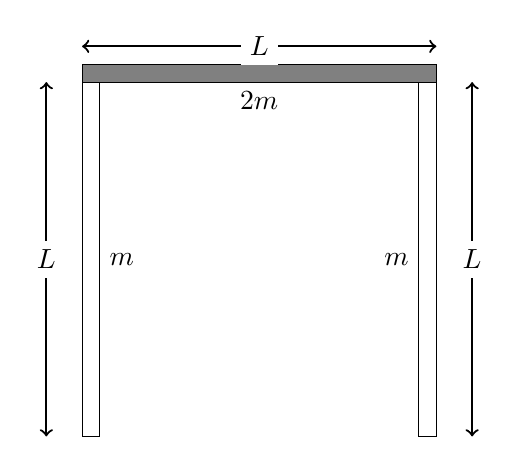
\begin{tikzpicture}[scale=1.50]
        %% Rods
        \draw (0,0) rectangle (1ex,-3cm);
        \draw[fill=white!50!black] (0,0) rectangle (3cm,+1ex);
        \draw (3cm,0) rectangle (3cm-1ex,-3cm);
        %% Mass
        \node[anchor=north] at (1.5cm,0) {$2m$};
        \node[anchor=west] at (1ex,-1.5cm) {$m$};
        \node[anchor=east] at (3cm-1ex,-1.5cm) {$m$};
        %% Length
        \draw[thick,<->] (0,2ex) -- (3cm,2ex) node[anchor=center,pos=0.5,fill=white] {$L$};
        \draw[thick,<->] (-2ex,0) -- (-2ex,-3cm) node[anchor=center,pos=0.5,fill=white] {$L$};
        \draw[thick,<->] (3cm+2ex,0) -- (3cm+2ex,-3cm) node[anchor=center,pos=0.5,fill=white] {$L$};
    \end{tikzpicture}
    \end{center}
    The two rods of the arms of the U each have mass $m$;
        the third rod has mass $2m$.
    How far below the midpoint of the horizontal rod is the center of mass of this assembly?
    \begin{multicols}{3}
    \begin{choices}
        \wrongchoice{$\dfrac{L}{8}$}
        \wrongchoice{$\dfrac{L}{4}$}
        \wrongchoice{$\dfrac{3L}{8}$}
        \wrongchoice{$\dfrac{L}{2}$}
        \wrongchoice{$\dfrac{3L}{4}$}
    \end{choices}
    \end{multicols}
\end{question}
}

\element{AP}{
\begin{question}{momentum-Q09}
A wooden block of mass $M$ is moving at speed $V$ in a straight line.
    \begin{center}
    \begin{tikzpicture}[scale=1.25]
        \draw (-3,0) -- (3,0);
        \draw[fill=white!50!black] (-2,2em) circle (3pt) node[anchor=south,yshift=0.25em] {$m$};
        \draw[thick,->] (-2,2em) -- ++ (0:2cm);
        \node[anchor=south,minimum size=4em,draw] (M) at (+2,0em) {$M$};
        \draw[thick,->] (M.north) ++(90:1ex) -- ++ (180:1cm) node[anchor=south,pos=0.5] {$V$};
    \end{tikzpicture}
    \end{center}
    How fast would the bullet of mass $m$ need to travel to stop the block
        (assuming that the bullet became embedded inside)?
    \begin{multicols}{3}
    \begin{choices}
        \wrongchoice{$\dfrac{mV}{m+M}$}
        \wrongchoice{$\dfrac{MV}{m+M}$}
        \wrongchoice{$\dfrac{mV}{M}$}
        \wrongchoice{$\dfrac{MV}{m}$}
        \wrongchoice{$\dfrac{(m+M)V}{m}$}
    \end{choices}
    \end{multicols}
\end{question}
}

\element{AP}{
\begin{question}{momentum-Q10}
    Which of the following best describes a perfectly inelastic collision free of external forces?
    \begin{choices}
        \wrongchoice{Total linear momentum is never conserved.}
        \wrongchoice{Total linear momentum is sometimes conserved.}
      \correctchoice{Kinetic energy is never consersed.}
        \wrongchoice{Kinetic energy is sometimes consersed.}
        \wrongchoice{Kinetic energy is always consersed.}
    \end{choices}
\end{question}
}


\endinput


